\documentclass{beamer}

% This file is a solution template for:

% - Talk at a conference/colloquium.
% - Talk length is about 20min.
% - Style is ornate.

\mode<presentation>
{
  \usetheme{Dresden}
  % or ...

  \setbeamercovered{transparent}
  % or whatever (possibly just delete it)
}


\usepackage[english]{babel}
% or whatever

%\usepackage[latin1]{inputenc}
% or whatever

%\usepackage{times}
%\usepackage[T1]{fontenc}
% Or whatever. Note that the encoding and the font should match. If T1
% does not look nice, try deleting the line with the fontenc.

\usepackage{listings}
%numbers=left,
%numbersep=0pt,
\lstset{language=Java, basicstyle=\footnotesize, indent=xleftmargin}


\title %[Taming XML] % short title
{Taming XML: Objects First, Then Markup}

%\subtitle
%{Include Only If Paper Has a Subtitle}

\author[Bone, Nabicht, L\"{a}ufer, Thiruvathukal] % (short authors list)
{Matt Bone, Peter F. Nabicht, Konstantin L\"{a}ufer,\\and George K. Thiruvathukal}
% - Give the names in the same order as the appear in the paper.
% - Use the \inst{?} command only if the authors have different
%   affiliation.

\institute[Loyola University Chicago] % (optional, but mostly needed)
{
  %\inst{1}%
  Emerging Technologies Laboratory\\
  Department of Computer Science \\
  Loyola University Chicago
}


% - Use the \inst command only if there are several affiliations.
% - Keep it simple, no one is interested in your street address.

\date[EIT 2008] % (optional, should be abbreviation of conference name)
{2008 IEEE International Conference\\on Electro/Information Technology}
% - Either use conference name or its abbreviation.
% - Not really informative to the audience, more for people (including
%   yourself) who are reading the slides online

% If you have a file called "university-logo-filename.xxx", where xxx
% is a graphic format that can be processed by latex or pdflatex,
% resp., then you can add a logo as follows:

% \pgfdeclareimage[height=0.5cm]{university-logo}{university-logo-filename}
% \logo{\pgfuseimage{university-logo}}

% Delete this, if you do not want the table of contents to pop up at
% the beginning of each subsection:
%\AtBeginSubsection[]
%{
%  \begin{frame}<beamer>{Outline}
%    \tableofcontents[currentsection,currentsubsection]
%  \end{frame}
%}


% If you wish to uncover everything in a step-wise fashion, uncomment
% the following command: 

%\beamerdefaultoverlayspecification{<+->}


\begin{document}

\begin{frame}
  \titlepage
\end{frame}

%\begin{frame}{Outline}
%  \tableofcontents
%  % You might wish to add the option [pausesections]
%\end{frame}


% Structuring a talk is a difficult task and the following structure
% may not be suitable. Here are some rules that apply for this
% solution: 

% - Exactly two or three sections (other than the summary).
% - At *most* three subsections per section.
% - Talk about 30s to 2min per frame. So there should be between about
%   15 and 30 frames, all told.

% - A conference audience is likely to know very little of what you
%   are going to talk about. So *simplify*!
% - In a 20min talk, getting the main ideas across is hard
%   enough. Leave out details, even if it means being less precise than
%   you think necessary.
% - If you omit details that are vital to the proof/implementation,
%   just say so once. Everybody will be happy with that.

%\section{Motivation}
\begin{frame}{Motivation}
The BetterXML framework aims to:
\begin{itemize}
  \item Minimize the accidental complexity of handling XML 
  \item Focus on the domain objects and  bind to XML later
\end{itemize}
\end{frame}

\begin{frame}{A Guiding Example}
  Thinking of a simple calculator, we can represent a calculation like 
  $21+20+(5-4)$ as an expression tree:

  \begin{center}\includegraphics[height=6cm]{expression_tree}\end{center}
\end{frame}

\begin{frame}{Expression Tree In an Object Oriented Language}
  \begin{center}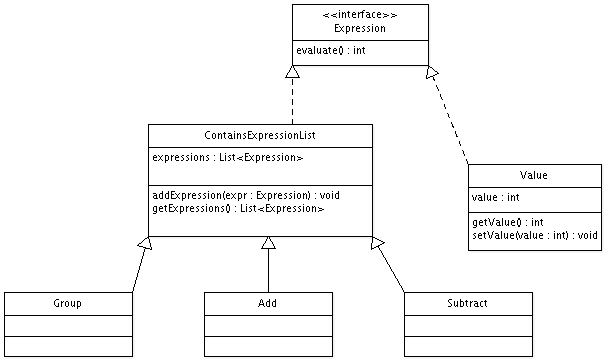
\includegraphics[height=6cm]{expr_tree_diagram}\end{center}
\end{frame}

%\begin{frame}[fragile]{Expression Tree In an Object Oriented Language}
%  \begin{lstlisting}
%  public interface Expression {
%    public int evaluate();
%  }
%
%  public class Add {
%  //insert code here.
%  }
%  \end{lstlisting}
%\end{frame}

\begin{frame}[fragile]{Expression Tree as Markup}
  %Markup is tree oriented!
  \begin{lstlisting}
    <group>
      <add>
        <value value="21"/>
        <value value="20"/>
        <subtract>
          <value value="5"/>
          <value value="4"/>
        </subtract>
      </add>
    </group>
  \end{lstlisting}
\end{frame}

\begin{frame}[fragile]{Mapping the Expression Tree to Markup with XElement}
\begin{lstlisting}
public class Add extends XElement implements Expression{
  
  public int evaluate() {
    int result=0;
    
    for (XElement element: this.getChildrenElements()) {
      if (element instanceof Expression) 
      result += ((Expression) element).evaluate();
    }
    
    return result;
  }
}
\end{lstlisting}
\end{frame}

\begin{frame}[fragile]{Mapping the Expression Tree to Markup with XElement}
Using XElement is quite similar except that individual classes
may be bound to individual elements:
\begin{lstlisting}
ToXElementContentHandler handler = 
    new ToXElementContentHandler();
handler.registerElementClass(Add.class, "add");
handler.registerElementClass(Subtract.class, "subtract");
handler.registerElementClass(Group.class, "group");
handler.registerElementClass(Value.class, "value");
\end{lstlisting}
\end{frame}

\begin{frame}[fragile]{Mapping the Expression Tree to Markup with NaturalXML}
  \begin{lstlisting}
@Element("add")
public class Add extends ContainsExpressionList {
  
  public int evaluate() {
    int sum = 0;
    
    for(Expression expression: expressions) {
      sum += expression.evaluate();
    }
    
    return sum;
  } 
}
\end{lstlisting}
\end{frame}

\begin{frame}[fragile]{Mapping the Expression Tree to Markup with NaturalXML}
\begin{lstlisting}
public abstract class ContainsExpressionList 
   implements Expression {
    
  @Children({Group.class, Add.class, 
    Subtract.class, Value.class})
  protected List<Expression> expressions = 
    new ArrayList<Expression>();
  
  public List<Expression> getExpressions() {
    return expressions;
  }
  
  public void addExpression(Expression expression) {
    this.expressions.add(expression);
  }
}
\end{lstlisting}
\end{frame}

\begin{frame}[fragile]{Mapping the Expression Tree to Markup with NaturalXML}
\begin{lstlisting}
@Element("value")
public class Value implements Expression {
	
  @Attribute("value")
  private String value;
  
  public String getValue() { return value; }
  public void setValue(String value) { this.value = value; }
  
  public int evaluate() {
    return Integer.valueOf(value);
  }
}
\end{lstlisting}
\end{frame}

\begin{frame}{NaturalXML Annotations}
NaturalXML allows the binding of elements to classes with class metadata:
  \begin{itemize}
    \item @Element
    \item @Attribute
    \item @Children
    \item @CData
    \item @Singleton
    \item @Namespace
  \end{itemize}
\end{frame}

%Plain Old Object Hierarchies (POOHs)
%Working without XML (where XIR comes in)
\begin{frame}{XML Intermediate Representation (XIR)}
\begin{itemize}
  \item A record oriented, lossless representation of XML
  \item Character data encoded as Base64
  \item Easy to parse
\end{itemize}
\end{frame}

\begin{frame}[fragile]{Some Simple XML...}
\begin{lstlisting}
<value value="5">some cdata</value>
\end{lstlisting}
\end{frame}

\begin{frame}[fragile]{...translated to XIR}
\begin{lstlisting}
xir.type:verbatim=element
ns:verbatim=
xir.subtype:verbatim=begin
qname:verbatim=value
name:verbatim=value
attributes:verbatim=1

xir.type:verbatim=attribute
ns:verbatim=
xir.subtype:verbatim=none
qname:verbatim=value
name:verbatim=value
value:verbatim=5

xir.type:verbatim=characters
cdata:base64=c29tZSBjZGF0YQ==
xir.subtype:verbatim=none
length:verbatim=10

xir.type:verbatim=element
ns:verbatim=
xir.subtype:verbatim=end
qname:verbatim=value
name:verbatim=value
\end{lstlisting}
\end{frame}

%\begin{frame}{Related Work}
%  ...
%\end{frame}

\begin{frame}{Future Directions}
\begin{itemize}
  \item XElement expressed as a subset of NaturalXML
  \item Various Input/Output formats: YAML, s-expressions
  \item RelaxNG Schema to BetterXML transformer
  \item Interesting applications: BetterPipes
\end{itemize}
Any questions?
\end{frame}

\begin{frame}{Availability}
  The BetterXML framework can be downloaded at: \url{http://betterxml.googlecode.com}
\end{frame}

\end{document}


